\section{Cylc Overview}

Cylc ("silk") is a workflow scheduling tool of particular use in cycling
environmental forecasting suites. Cylc understands workflows as collections of
inter-dependent tasks for example the following diagram shows an example
workflow as seen by cylc.

\begin{center}
    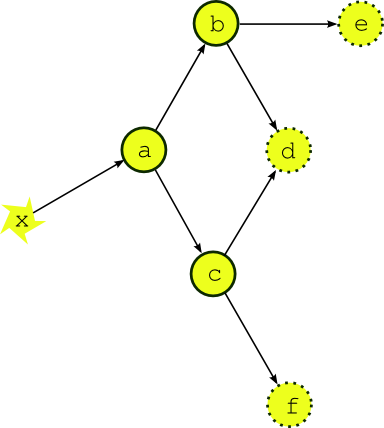
\includegraphics[width=0.4\columnwidth]{resources/tex/dep-one-cycle}
\end{center}
Cylc employs a novel self-organising scheduling algorithm for running
workflows that is simple but powerful. Each task knows its own
inputs and outputs, tasks run as soon as their inputs are satisfied. The
following diagram shows how cylc would run the previous example.

\begin{center}
    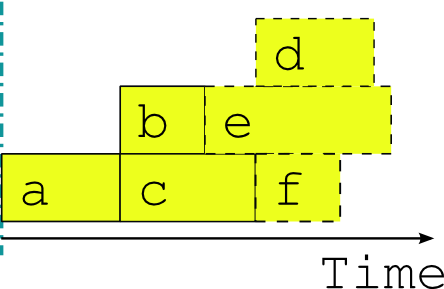
\includegraphics[width=0.3\columnwidth]{resources/tex/timeline-zero.png}
\end{center}

In most applications we want to repeat workflows over time (cycling).

\begin{center}
    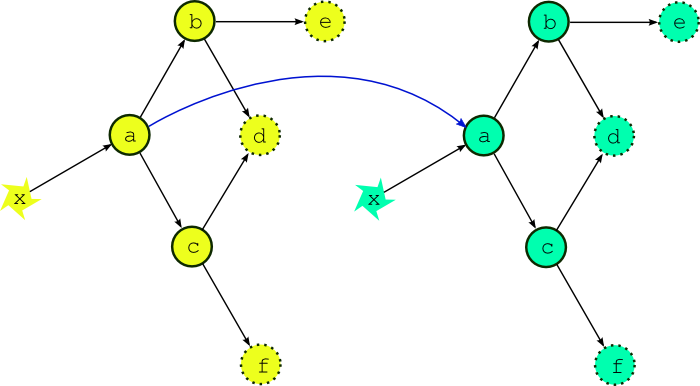
\includegraphics[width=0.5\columnwidth]{resources/tex/dep-two-cycles-linked}
\end{center}

Cylc runs tasks as soon as their inputs are satisfied irrespective of which
cycle they are in, that is to say if a task can run ahead of its cycle time it
should. This means that suites can make a head start on the next cycle before
finishing the previous. This behaviour makes cylc able to run workflows
faster, recover from outages quicker and handle failed tasks better. The
following diagram outlines the difference between cylc (top) and a traditional
cycle-fixed scheduler (bottom) for the previous example workflow cycling
many times.

\begin{center}
    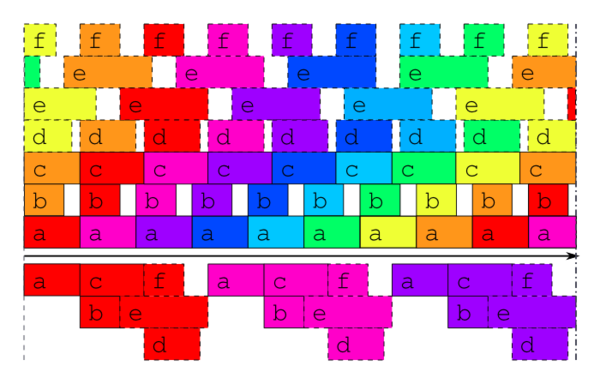
\includegraphics[width=0.6\columnwidth]{resources/tex/timeline-two}
\end{center}
